%%!
% @file 01_introduction.tex
% @brief Template for Chapter 1 demonstrating heading hierarchy, lists, tables, figures, and code.

\chapter{Tiêu đề chương 1}
\label{chap:chapter_1}

Đây là nội dung mở đầu của chương 1 trong bản mẫu báo cáo. Đoạn văn bản này minh họa định dạng chuẩn với cỡ chữ 13pt, khoảng cách giãn dòng 1.5 và thụt đầu dòng 1.25cm theo quy định kỹ thuật \cite{doe2023}. Nội dung mẫu có thể được thay thế bằng phần giới thiệu tổng quan, bối cảnh thực hiện hoặc mục tiêu nghiên cứu của đề tài.

Lorem ipsum dolor sit amet, consectetur adipiscing elit. Sed do eiusmod tempor incididunt ut labore et dolore magna aliqua. Ut enim ad minim veniam, quis nostrud exercitation ullamco laboris nisi ut aliquip ex ea commodo consequat \cite{newman2021}.

\section{Tiêu đề mục 1.1}
\label{sec:section_1_1}

Nội dung chi tiết của mục 1.1 trình bày cơ sở lý luận, bối cảnh hoặc các vấn đề trọng tâm liên quan đến nội dung chương 1. Dưới đây là các tiểu mục được phân cấp chi tiết.

\subsection{Tiêu đề mục 1.1.1}
\label{subsec:subsection_1_1_1}

Nội dung minh họa của mục 1.1.1. Đoạn này minh họa cách trình bày danh sách hoa thị đa cấp theo chuẩn định dạng kỹ thuật:

\begin{itemize}
    \item Nội dung danh sách cấp 1 -- Mục thứ nhất (sử dụng dấu gạch ngang, khoảng cách lề trái chuẩn).
    \item Nội dung danh sách cấp 1 -- Mục thứ hai với các ý chi tiết bên trong:
          \begin{itemize}
              \item Nội dung danh sách cấp 2 -- Chi tiết 2.1 (sử dụng ký hiệu dấu cộng, thụt đầu dòng 1.25cm).
              \item Nội dung danh sách cấp 2 -- Chi tiết 2.2.
          \end{itemize}
    \item Nội dung danh sách cấp 1 -- Mục thứ ba.
\end{itemize}

\subsubsection{Tiêu đề mục 1.1.1.1}
\label{subsubsec:subsubsection_1_1_1_1}

Nội dung minh họa cấp đề mục thứ 4 (Sub-subsection) với tiền tố số 4 cấp. Theo đặc tả mẫu, cấp này chỉ hiển thị trong nội dung chính và tự động không xuất hiện trong Mục lục để đảm bảo tính tinh gọn của tài liệu.

\section{Tiêu đề mục 1.2}
\label{sec:section_1_2}

Mục này minh họa quy cách trình bày các đối tượng nổi (floats) bao gồm bảng biểu và hình vẽ, cùng cơ chế tham chiếu chéo tự động. Bảng \ref{tab:sample_table} minh họa bảng dữ liệu mẫu có đệm 4pt trên và dưới.

%%!
% @brief Example table demonstrating the use of tabularx and custom column types in LaTeX.

\begin{table}[h!]
    \caption{Tiêu đề bảng 1.1}
    \label{tab:sample_table}
    \centering
    \begin{tabularx}{\textwidth}{|C{1.5cm}|Y|C{3.0cm}|C{3.0cm}|}
        \hline
        \thcell{STT} & \thcell{Tiêu chí đánh giá mẫu} & \thcell{Thông số A} & \thcell{Thông số B} \\ \hline
        1            & Dữ liệu thử nghiệm mẫu số 01   & 100                 & 200                 \\ \hline
        2            & Dữ liệu thử nghiệm mẫu số 02   & 300                 & 400                 \\ \hline
        3            & Dữ liệu thử nghiệm mẫu số 03   & 500                 & 600                 \\ \hline
    \end{tabularx}
\end{table}

Bên cạnh bảng biểu, Hình \ref{fig:sample_figure} minh họa một sơ đồ khối kỹ thuật được vẽ trực tiếp bằng gói lệnh TikZ với chú thích căn giữa bên dưới hình ảnh.

\begin{figure}[h!]
    \centering
    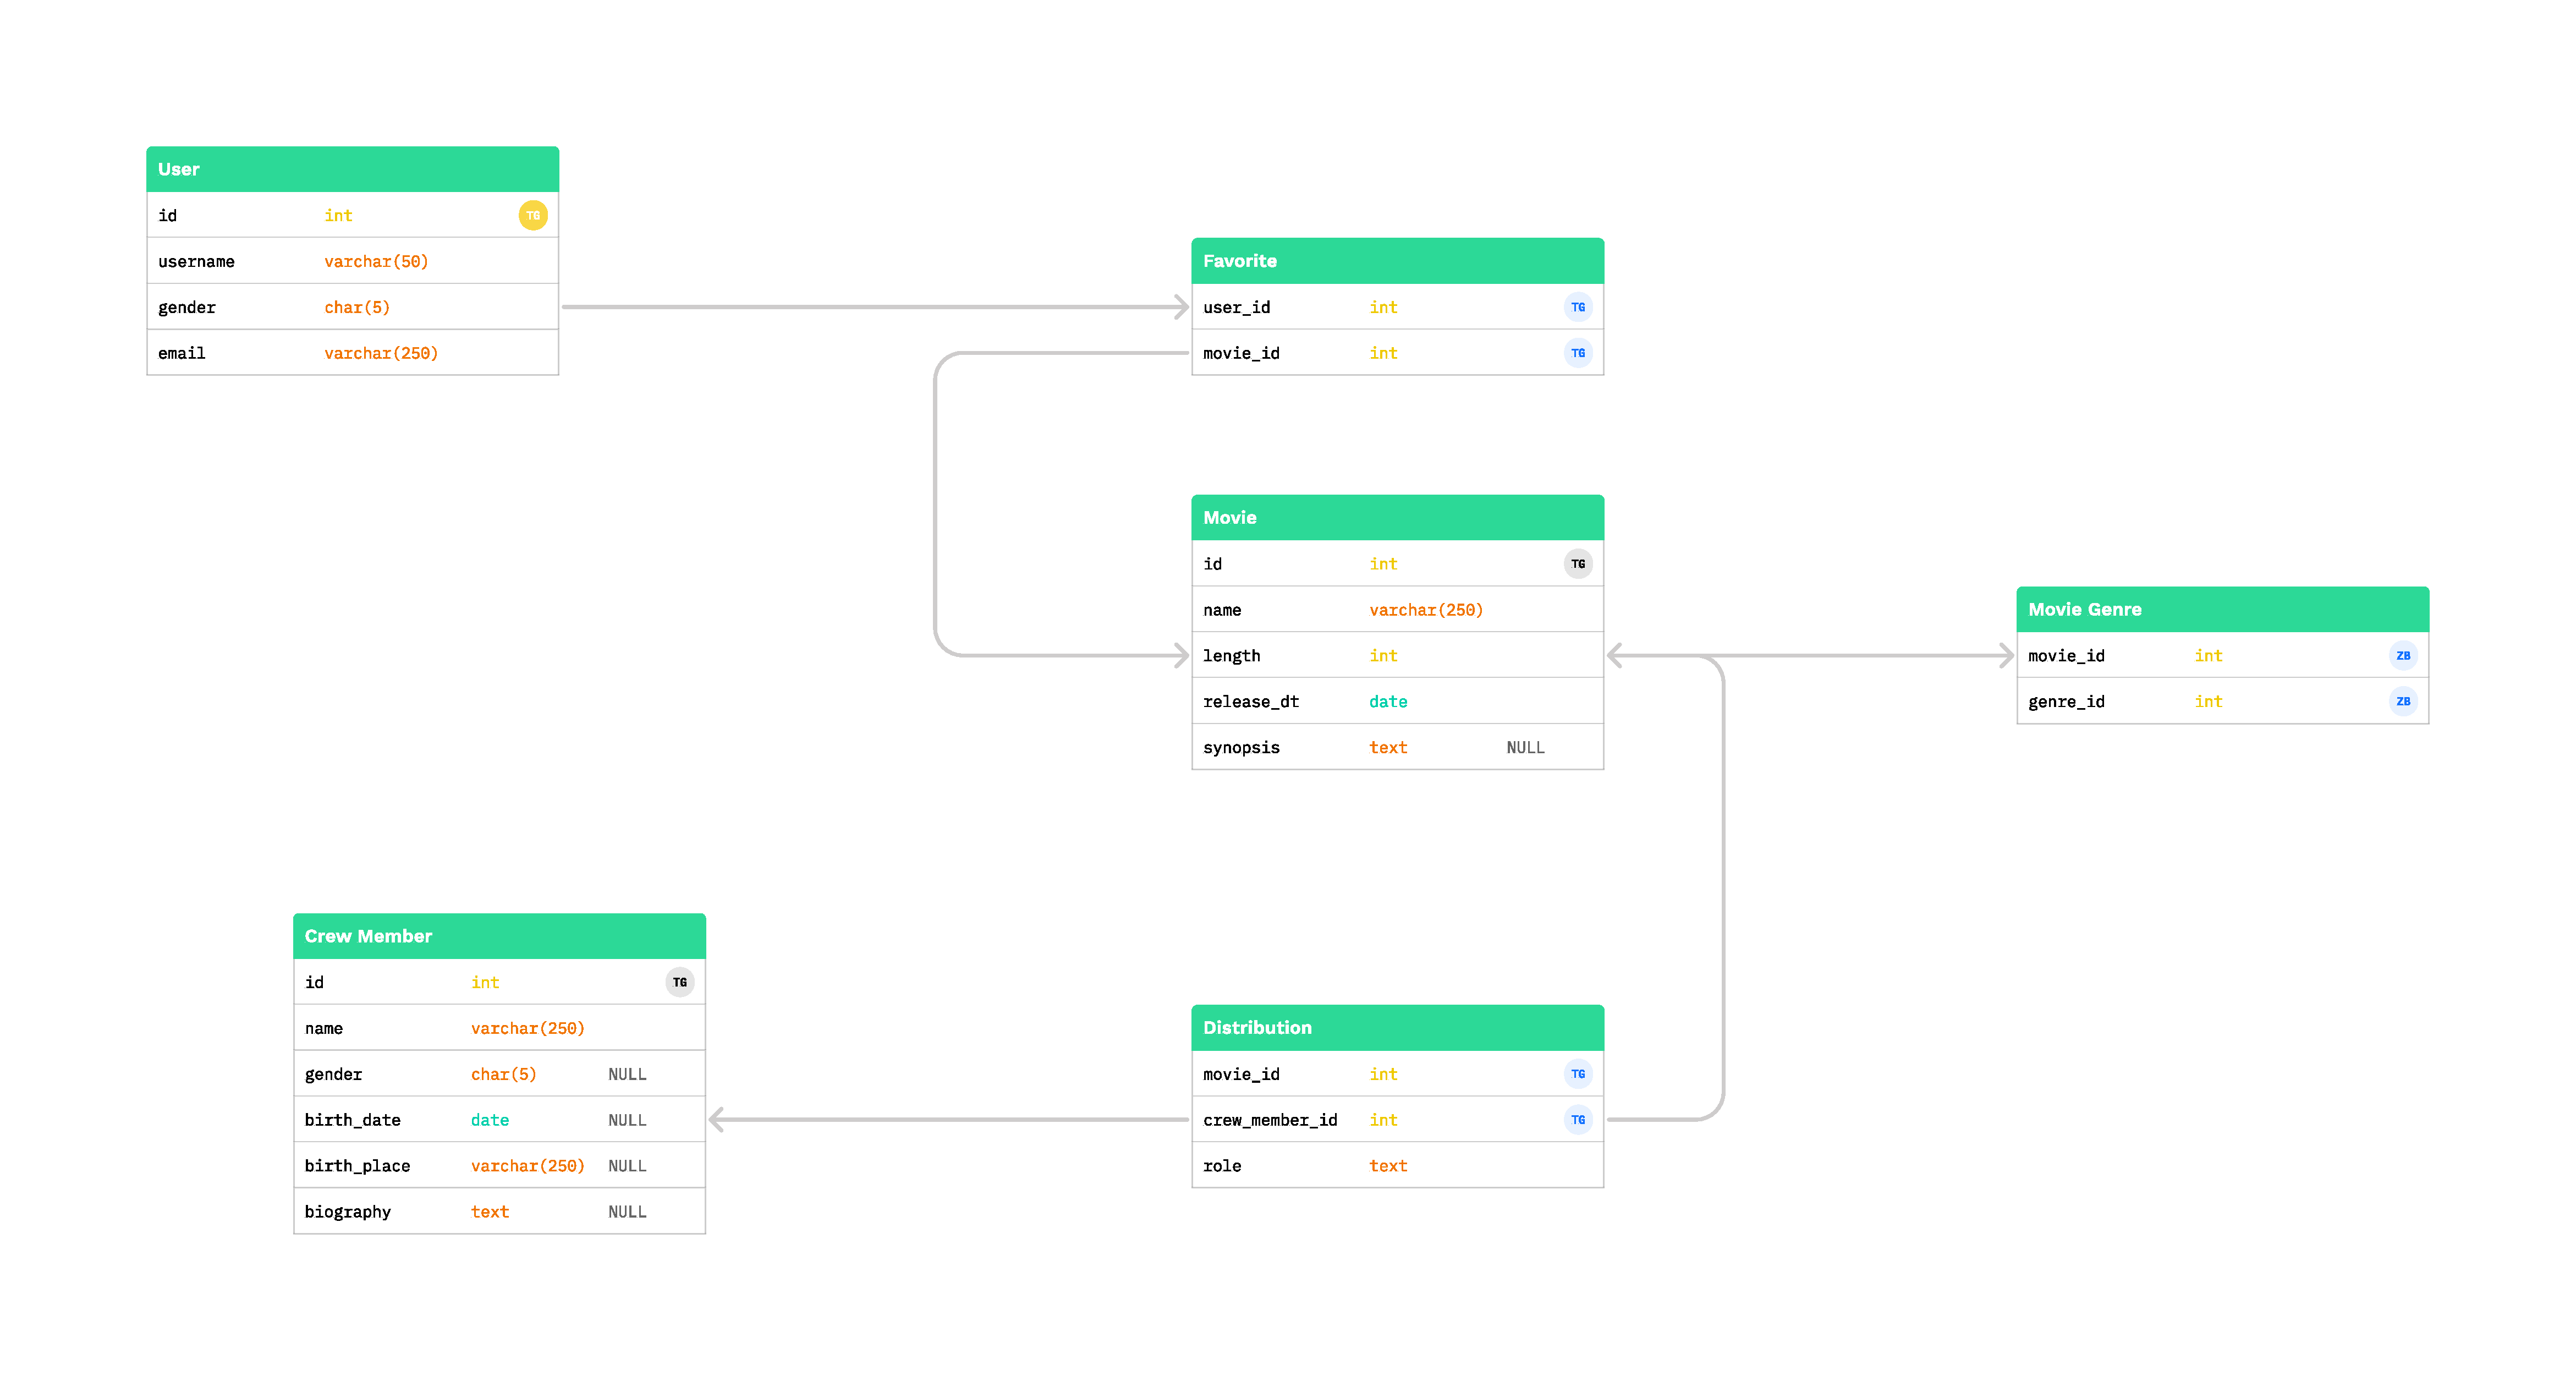
\includegraphics[width=\textwidth, height=0.7\textheight, keepaspectratio]{assets/figures/ch01/example_figure.pdf}
    \caption{Tiêu đề hình 1.1}
    \label{fig:sample_figure}
\end{figure}

\section{Tiêu đề mục 1.3}
\label{sec:section_1_3}

Đoạn mã sau minh họa cách trình bày khối mã nguồn hệ thống với định dạng hộp viền đơn, cỡ chữ 10pt phông Inconsolata, như được hiển thị tại Đoạn mã \ref{lst:sample_code}.

\begin{lstlisting}[language=Python, caption={Tiêu đề đoạn mã 1.1}, label={lst:sample_code}]
def example_function(param_a: int, param_b: int) -> int:
    """Tinh tong hai so nguyen va tra ve ket qua."""
    result = param_a + param_b
    return result

if __name__ == "__main__":
    output = example_function(10, 20)
    print(f"Ket qua tinh toan: {output}")
\end{lstlisting}
